%        File: main.tex
%     Created: 日 10月 27 08:00 下午 2019 C
% Last Change: 日 10月 27 08:00 下午 2019 C
%
\documentclass{ctexart}
\usepackage[a4paper,left=3.2cm,right=3.2cm,top=2.8cm,bottom=2.8cm]{geometry}
\usepackage{fancyhdr}
\usepackage{setspace}
\usepackage{hyperref}
\usepackage{url}
\usepackage{cite}
\usepackage{graphicx}
\usepackage{amsmath}
\usepackage{amssymb}
\usepackage{enumitem}
\usepackage{tikz}
\usepackage{float}
\usepackage{listings}
\usepackage{xcolor}
\usepackage{forest}
\usepackage{pgf}
\usepackage{multirow}
\usepackage{extarrows}
\usetikzlibrary{graphs}
\usetikzlibrary{arrows,automata}
\lstset{language = c,numbers=left, showstringspaces = false, keywordstyle= \color{ blue!70 },commentstyle=\color{red!50!green!50!blue!50}, frame=shadowbox, rulesepcolor= \color{ red!20!green!20!blue!20 } 
} 

\CTEXsetup[format={\Large\bfseries}]{section}
\pagestyle{fancy}

\lhead{中国科学院大学}
\rhead{图神经网络综述}

\cfoot{\thepage}
\usetikzlibrary{graphs}
\renewcommand{\baselinestretch}{1.0}
\title{图神经网络综述}
\author{\begin{tabular}{ll}冯吕 & $201928013229158$\\
	张佳锋 & $2019xxxxxxxxxxx$
\end{tabular}}
\date{}

\begin{document}
\bibliographystyle{IEEEtran}
\maketitle
\zihao{-4}
\CJKfamily{zhsong}
\begin{abstract}
 这是摘要\\

\centering
\textbf{关键字:}图神经网络、Node Embedding、RGNN、GCN、Graph Generation
\end{abstract}

参考文献测试:引用\cite{grover2016node2vec}
\usepackage{CJK}

\section{背景}
近年来,深度学习在许多机器学习任务上取得了革命性的进展,比如图像分类、视频处理、语音识别、自然语言理解等。深度学习在这些领域的成功部分归因于快速发展的计算资源(如GPU),大量训练数据的可用性,以及深度学习从欧几里得数据抽取特征表示的有效性。图像、文本和视频等均可表示为欧几里得空间中的数据。以图像为例,我们可以将图像表示为欧几里得空间中的规则网络,卷积神经网络(GNN)\cite{NIPS2012_4824}能够利用图像数据的平移不变形,局部连通性和合成性,从而提取与整个数据集共享的局部特征,以进行各种图像分析。

与此同时,图(Graph)数据易于描述对象之间的复杂关系,因此越来越来的任务用图结构来表示数据,比如社交网络、推荐系统以及知识图谱等。以社交网络为例,在社交网络图中,节点表示个人或组织,而边表示节点之间的各种关系,通过对社交网络进行挖掘,能够发现虚拟社区,进行用户行为分析等。然而,图数据的复杂性对现有的机器学习算法提出了重大挑战。由于图具有复杂的拓扑结构,没有固定的节点顺序,并且图可能是动态的,因此一些重要的操作例如卷积,在图像域中易于计算,但是应用于图域却非常困难。此外,现有机器学习算法的核心假设是实例彼此独立,但是该假设不再适用于图数据,因为每个实例(节点)通过引用、朋友关系等各种类型的链接与其它实例相关联。

为了应对图数据问题的复杂性,图表示学习应运而生。图数据本身是非欧几里得空间的数据,为了能够将传统的机器学习方法运用到图数据上,我们需要将图数据表示成欧几里得空间中的数据,而这正是图表示学习所研究的内容。受自动编码器(Auto-encoder)\cite{hinton2006reducing}和词嵌入(Word-Embedding)\cite{mikolov2013distributed} 的启发,我们希望能够将网络中的节点表示为特征向量,使得该向量能够自带节点信息,例如在特征空间上,相似的节点会离得特别近,这将有利于机器学习的任务

在图表示学习中,给定一个图$G(V, E, W)$,其中,$V$是节点集,$E$是节点之间的边集,$W$是边上的权重集合,我们通过embedding方法将每一个节点表示成一个$d$维向量,简单来说就是将节点映射成低维向量,如图\ref{fig:nodeed}所示。更具体地说,图表示学习由两个关键部分组成:
\begin{itemize}
  \item 编码器(encoder):将每一个节点映射成一个低维向量。
	\[\text{ENC}(v) = \textbf{Z}_v\]
	其中,$v$是图中的节点,$\textbf{Z}_v$是一个$d$维向量。
	\item 相似度(similarity)函数:指定向量空间中的向量关系如何映射到原图中节点之间的关系。
	  \[\text{similarity}(u, v) \approx \textbf{z}_v^T\textbf{z}_u\]
	  其中,$\text{similarity}(u, v)$表示$u, v$两个节点在图中的相似度,$\textbf{z}_v^T \textbf{z}_u$表示两个节点向量的点积。该公式也正是图表示学习的优化目标。
\end{itemize}

\begin{figure}[!htbp]
  \centering
  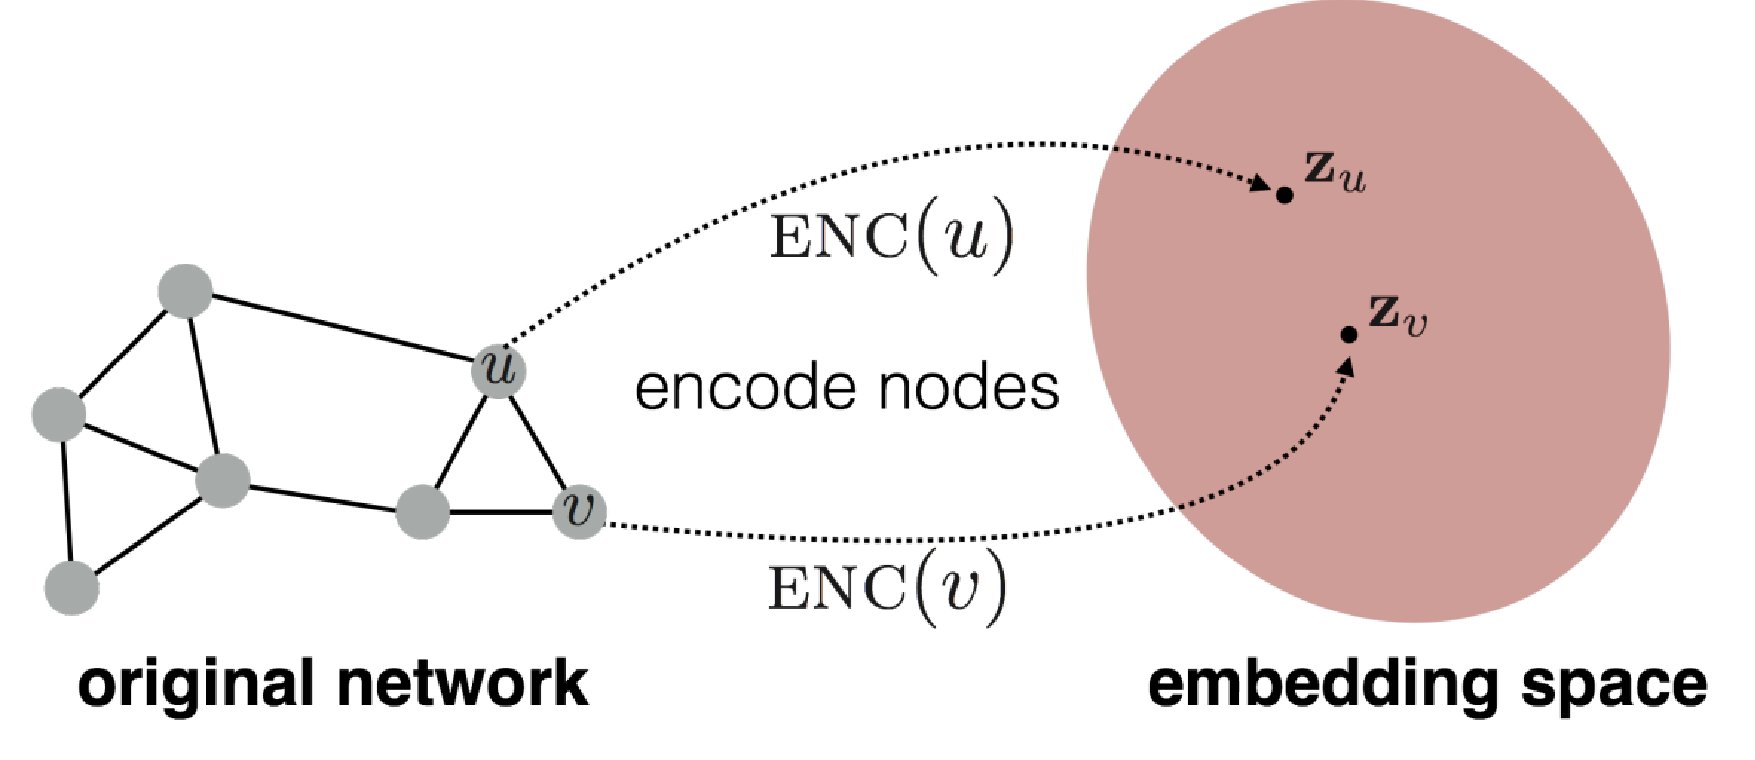
\includegraphics[width=\textwidth]{Fig/nodeem.pdf}
  \caption{Node embedding:将节点映射到低维向量空间}
  \label{fig:nodeed}
\end{figure}

最简单的编码器就是如下一个embedding表:
\[\text{ENC}(v) = \textbf{Z}_\textbf{v}\]
其中,$\textbf{Z}$是$R^{d\times |V|}$ 维的矩阵,每一列是一个节点向量,\textbf{v}是一个指示符向量,向量中只有一个位置为1,其余位置全为0,因此,每一个节点映射到一个唯一的特征向量。这一类编码方法有LINE\cite{tang2015line}、DeepWalk\cite{perozzi2014deepwalk}和Node2vec\cite{grover2016node2vec}等,而这些方法的主要区别在于节点相似度如何定义。

然而,上面谈到的这一类简单的node embedding方法存在如下一些弊端:首先,由于每一个节点被映射到一个唯一的特征向量,并且节点之间没有参数共享,因此,总要需要$O(|V|)$个参数;其次,由上文的介绍容易知道,该方法仅能对训练过程中出现的节点进行编码,而无法编码训练过程中从未出现过的节点;另外,无法合并节点特征。因此,我们需要提出一些更加"Deep"的node embedding方法,这就是图神经网络(GNN)。

图神经网络使用更加复杂的函数来对节点进行编码,对一个节点进行编码时通常还需要用到其邻居节点的信息。在本文中,我们沿用Wu等(2019)\cite{wu2019comprehensive}提出的图神经网络分类方法,主要将GNN分为如下四类:
\begin{itemize}
  \item 循环图神经网络(RecGNN):RecGNN旨在通过循环神经网络架构来学习节点表示,该网络假设图中的节点能够持续地与邻居节点交换信息,直到达到稳定平衡点。
\item 卷积图神经网络(ConvGNN):ConvGNN将卷积操作从网格数据泛化到了图数据上,其主要思想是通过汇总节点自身的特征\textbf{x}$_v$和邻居节点的特征\textbf{x}$_u$来学习节点的表示。
  \item 图自动编码器(GAE):GAE是一种无监督学习方法,其能够将节点或图编码到特征向量空间,并从编码信息中重构图信息。
	\item 时空图神经网络(STGNN):STGNN旨在从时空图中学习隐藏模式。
\end{itemize}

\begin{figure}[!htbp]
  \centering
  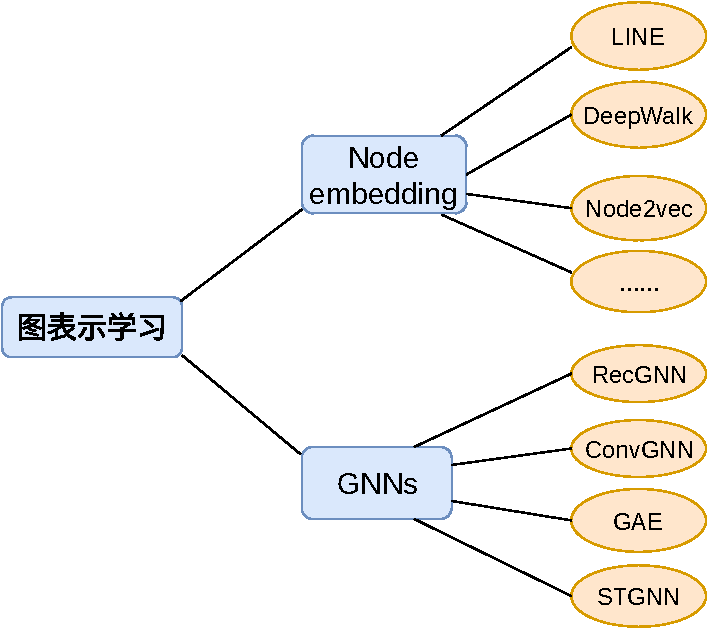
\includegraphics[scale = 1]{Fig/gnn.pdf}
  \caption{图表示学习分类树状图}
  \label{fig:gnn}
\end{figure}

图\ref{fig:gnn}是图表示学习的分类树状图,正如上文所谈到的,图神经网络是将深度学习方法应用到图表示学习的一种高级方法,也是本文阐述的重点。在本文的第二部分,我们将对普通的典型node embedding包括LINE、DeepWalk和Node2vec进行简要介绍;在第三部分,我们将重点介绍图\ref{fig:gnn}中的四种不同类别的图神经网络;最后,我们将对图表示学习和图神经网络当前的实际应用以及当前面临的困难和挑战进行简要介绍。



%reference
\bibliography{./Bib/ref}
\end{document}


